\documentclass{ximera}
\graphicspath{     %% setup a global graphics path
{./}               %% look in the same-level directory
{./pictures/}      %% look in graphics
{../pictures/}     %% look up one directory, then in graphics
%{../../pictures/} %% look up two directories, then in graphics
}

\author{Zack Reed}
%borrowed from mooculus calculus 2 https://ximera.osu.edu/mooculus/calculus2/differentialEquations/digInDifferentialEquations.tex
\title{Learning Activity: }
\begin{document}
\begin{abstract}


\end{abstract}
\maketitle

\section{Derivatives and Differential Equations}

A \textit{differential equation}\index{differential equation} is
simply an equation involving functions and their derivatives. Here is an example:
\[
2\cdot \frac{d^2f}{dx^2} + 3\cdot \frac{df}{dx} + 3\cdot f = g.
\]

You might in words say that ``A function $f$ satisfies the differential equation if twice its second-derivative plus three times its first derivative plus three times itself equals another function $g$''

\begin{question}
  What is a differential equation?
  \begin{multipleChoice}
    \choice{An equation that you take the derivative of.}
    \choice[correct]{An equation that relates the rates of a function to other values.}
    \choice{It is a formula for the slope of a tangent line at a given point.} 
  \end{multipleChoice}
\end{question}

When we solve differential equations, we find
\textit{functions} satisfying the equation.
\begin{question}
  Which of the following functions solve the differential equation
  \[
  \frac{d^4f}{dx^4} = f?
  \]

  \begin{hint}
    Remember, $\frac{d^4f}{dx^4}$ is the fourth derivative of $f$.
  \end{hint}

  \begin{selectAll}
    \choice[correct]{$f(x) = \sin(x)$}
    \choice{$f(x) = x^2$}
    \choice[correct]{$f(x) = e^x$}
    \choice[correct]{$f(x) = e^{-x}$}
    \choice{$f(x) = \tan(x)$}
  \end{selectAll}
  \begin{feedback}
    ANY function that is the same as its 4th derivative satisfies the equation. 
    In fact, we can combine all possible allowed functions from the list above to make a very general solution: $c_1\sin(x)+c_2\cos(x)+c_3e^x+c_4e^{-x}$.  
    
    In other words, every
    solution to this differential equation can be written in this form.
    You should check that these are all solutions (for example $f(x) =
    \sin(x)+3\cos(x)-7e^x+\pi e^{-x}$ is a solution). 
  \end{feedback}
\end{question}

We get more specific solutions to differential equations when we add \emph{boundary conditions}. That is, we specify the values at which the solution function starts and stops and then solve for the function values in between the boundary points. 

Let's specify some boundary conditions 

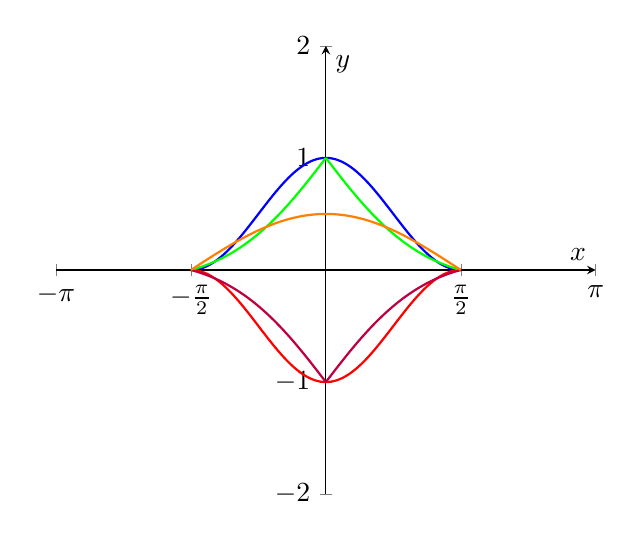
\begin{tikzpicture}
    \begin{axis}[
        domain=-pi:pi,
        samples=200,
        axis lines=middle,
        xlabel={$x$},
        ylabel={$y$},
        xtick={-3.1416, -1.5708, 1.5708, 3.1416},
        xticklabels={$-\pi$, $-\frac{\pi}{2}$, $\frac{\pi}{2}$, $\pi$},
        ytick={-2, -1, 0, 1, 2},
        %grid=major,
        xmin=-pi, xmax=pi,
        ymin=-2, ymax=2,
        xmajorgrids=false % Disable grid lines for x-axis
    ]
    % Plot various functions restricted to -pi/2 to pi/2
    \addplot[blue, thick, domain=-pi/2:pi/2] {cos(deg(x))^2};

    \addplot[red, thick, domain=-pi/2:pi/2] {sin(deg(x))^2 - 1};

    \addplot[green, thick, domain=-pi/2:pi/2] {exp(-abs(x)) * cos(deg(x))};

    \addplot[purple, thick, domain=-pi/2:pi/2] {-exp(-abs(x)) * cos(deg(x))};

    \addplot[orange, thick, domain=-pi/2:pi/2] {0.5 * cos(deg(x))};

    % Add arrows pointing to -pi/2 and pi/2
    %\node[above left, black] at (2, 1) {Boundary Conditions};
    %\draw[->, black, thick] (2,.8) -- (-1.5708, 0);

    %\node[above right, black] at (2,1) {Boundary Conditions};
    %\draw[->, black, thick] (2,.8) -- (1.5708, 0);

    \end{axis}
\end{tikzpicture}

Here, the boundary conditions are that $f=0$ at $x=\frac{-\pi}{2}$ and $x=\frac{\pi}{2}$. As you can see, there are many functions that satisfy these boundary conditions, but fewer functions that also have the differential equation property $\frac{d^4f}{dx^4} = f$.

The unique group of functions satisfying both the boundary conditions and the differential equations are the functions $c\sin(x)$, constant multiples of the sine function.

\section{Approximating Derviatives}

As we'll see later, at times it's better (or necessary) to just approximate the derivative or function values rather than to work with abstractly stated differential equations and functions. We will be doing this later in reference to the heat equation and Poisson's equation. 

For our purposes, we want to approximate the derivative (and 2nd derivative as we'll see) using \emph{only values of f}. That we only use values of \emph{f} is important for our use of linear algebra, as this will let us set up and solve systems of equations to find our solutions.

For instance, if we break up $-\frac{\pi}{2}$ to $\frac{\pi}{2}$ into 6 intervals, we get the following grid along the $x$-axis and the corresponding function values along the graph.

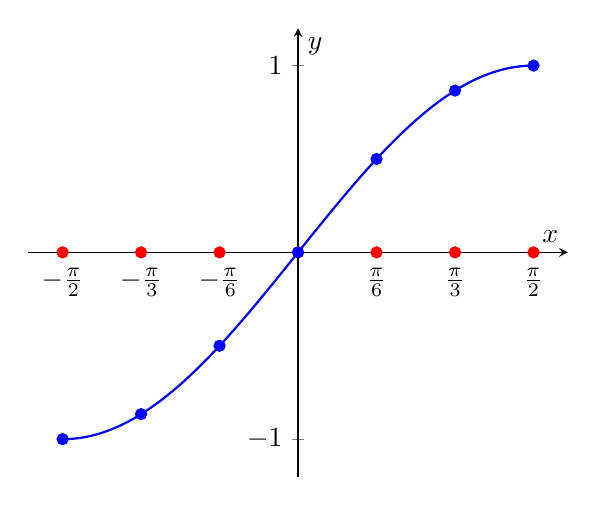
\begin{tikzpicture}
    \begin{axis}[
        domain=-1.5708:1.5708, % Limits for -pi/2 to pi/2 in radians
        samples=200,
        axis lines=middle,
        xlabel={$x$},
        ylabel={$y$},
        xtick={-1.5708, -1.0472, -0.5236, 0, 0.5236, 1.0472, 1.5708},
        xticklabels={$-\frac{\pi}{2}$, $-\frac{\pi}{3}$, $-\frac{\pi}{6}$, $0$, $\frac{\pi}{6}$, $\frac{\pi}{3}$, $\frac{\pi}{2}$},
        ytick={-1, 0, 1},
        xmin=-1.8, xmax=1.8,
        ymin=-1.2, ymax=1.2,
        grid=none,
    ]
    % Plot the sine function
    \addplot[blue, thick] {sin(deg(x))};

    % Add grid points on the x-axis
    \foreach \x in {-1.5708, -1.0472, -0.5236, 0, 0.5236, 1.0472, 1.5708} {
        \addplot[only marks, mark=*, mark options={red}] coordinates {(\x, 0)};
    }

    % Add grid points on the sine function
    \foreach \x in {-1.5708, -1.0472, -0.5236, 0, 0.5236, 1.0472, 1.5708} {
        \addplot[only marks, mark=*, mark options={blue}] coordinates {(\x, {sin(deg(\x))})};
    }

    \end{axis}
\end{tikzpicture}

If we wanted to approximate the derivative $\frac{d}{dx}\sin(x)$ around $\frac{\pi}{3}$, we could find the slope of the line connecting $\sin(\pi/6)$ and $\sin(\pi/2)$, as below.

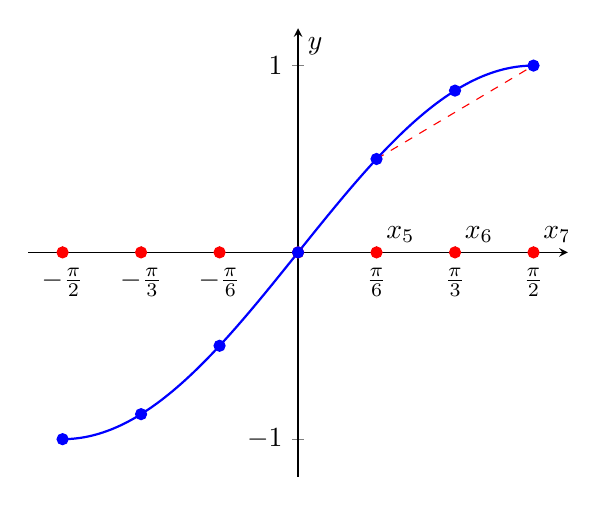
\begin{tikzpicture}
    \begin{axis}[
        domain=-1.5708:1.5708, % Limits for -pi/2 to pi/2 in radians
        samples=200,
        axis lines=middle,
        %xlabel={$x$},
        ylabel={$y$},
        xtick={-1.5708, -1.0472, -0.5236, 0, 0.5236, 1.0472, 1.5708},
        xticklabels={$-\frac{\pi}{2}$, $-\frac{\pi}{3}$, $-\frac{\pi}{6}$, $0$, $\frac{\pi}{6}$, $\frac{\pi}{3}$, $\frac{\pi}{2}$},
        ytick={-1, 0, 1},
        xmin=-1.8, xmax=1.8,
        ymin=-1.2, ymax=1.2,
        grid=none,
    ]
    % Plot the sine function
    \addplot[blue, thick] {sin(deg(x))};

    % Add grid points on the x-axis
    \foreach \x in {-1.5708, -1.0472, -0.5236, 0, 0.5236, 1.0472, 1.5708} {
        \addplot[only marks, mark=*, mark options={red}] coordinates {(\x, 0)};
    }

    % Add grid points on the sine function
    \foreach \x in {-1.5708, -1.0472, -0.5236, 0, 0.5236, 1.0472, 1.5708} {
        \addplot[only marks, mark=*, mark options={blue}] coordinates {(\x, {sin(deg(\x))})};
    }

    % Add labels for x_n, x_{n-1}, and x_{n+1}
    \node[above right] at (axis cs:1.0472, 0) {$x_6$};     % pi/3
    \node[above right] at (axis cs:0.5236, 0) {$x_{5}$}; % pi/6
    \node[above right] at (axis cs:1.5708, 0) {$x_{7}$}; % pi/2

    % Draw secant line between points on sine function from pi/6 to pi/2
    \addplot[red, dashed] coordinates {
        (0.5236, {sin(deg(0.5236))}) 
        (1.5708, {sin(deg(1.5708))})
    };
    \end{axis}
\end{tikzpicture}

We might say $\frac{d}{dx}\sin(x)|_{\pi/3}\approx \frac{\sin(\pi/2)-\sin(\pi/6)}{\pi/2-\pi/6}\approx .447465$. Compared to the exact value of the derivative $\frac{d}{dx}\sin(x)|_{\pi/3}=\cos(\pi/3)=.5$, this isn't too bad in the grand scheme of things, and would improve dramatically if we reduce the interval over which the derivative was approximated (i.e. $[\pi/6,\pi/2]$ is somewhat of a large interval for an approximation).

Notice that $\frac{\pi}{6}, \frac{\pi}{3}, $ and $\frac{\pi}{2}$ were labeled $x_5, x_6$ and $x_7$. This is becuase we broke the interval into $6$ subintervals, with $7$ points. Using this approximation technique, we can approximate the value of $\frac{d}{dx}f$ at an point $x_n$ with what is called the ``centered difference''

$$\frac{f(x_{n+1})-f(x_{n-1})}{2\Delta x},$$ 

where $\Delta x$ is the space between the grid points, as depicted below.

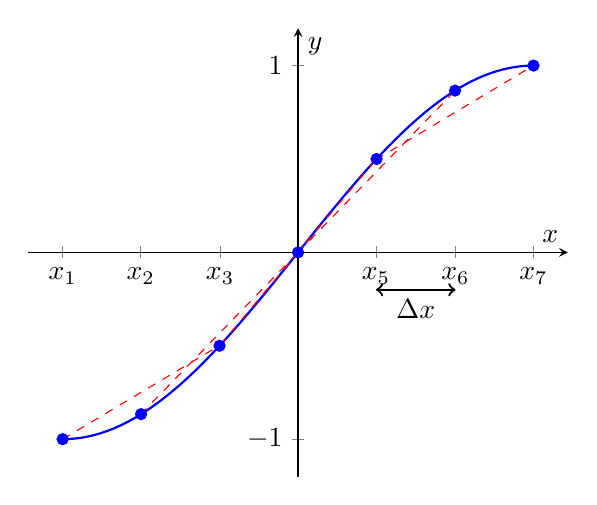
\begin{tikzpicture}
    \begin{axis}[
        domain=-1.57:1.57, % Approximation for -pi/2 to pi/2
        samples=200,
        axis lines=middle,
        xlabel={$x$},
        ylabel={$y$},
        xtick={-1.57, -1.05, -0.52, 0, 0.52, 1.05, 1.57},
        xticklabels={$x_{1}$, $x_{2}$, $x_{3}$, $x_{4}$, $x_{5}$, $x_{6}$, $x_{7}$},
        ytick={-1, 0, 1},
        xmin=-1.8, xmax=1.8,
        ymin=-1.2, ymax=1.2,
        grid=none,
    ]
    % Plot the sine function
    \addplot[blue, thick] {sin(deg(x))};

    % Draw secant lines between adjacent points
    \foreach \xA/\xB in {-1.57/-0.52, -1.05/0, 0/1.05, -0.52/0.52, 0.52/1.57} {
        \addplot[red, dashed] coordinates {
            (\xA, {sin(deg(\xA))})
            (\xB, {sin(deg(\xB))})
        };
    }

        % Add grid points on the sine function
        \foreach \x in {-1.5708, -1.0472, -0.5236, 0, 0.5236, 1.0472, 1.5708} {
            \addplot[only marks, mark=*, mark options={blue}] coordinates {(\x, {sin(deg(\x))})};
        }

    % Add \Delta x label between x_1 and x_2
    \draw[<->, thick] (axis cs:0.52, -0.2) -- (axis cs:1.05, -0.2);
    \node[below] at (axis cs:0.785, -0.2) {$\Delta x$};

    \end{axis}
\end{tikzpicture}

We can use Taylor Series (remember from Calc II?) to find a similar approximation of $\frac{d^2f}{dx^2}$ to be 

$$\frac{d^2f}{dx^2}\approx \frac{f(x_{n+1})-2f(x_n)+f(x_{n-1})}{\left(\Delta x\right)^2}.$$


\section{Derivatives and Differential Equations in Multiple Variables}

As much as we love the simplicity of single-variable calculus, the world is not so simple. Luckily, some ideas generalize fairly intuitively, such as the idea of a function of two or more variables, and derivatives in the directions of the variables $x$ and $y$. 

While there is much more nuance to unpack here, a summary of the ideas are as follows:

A function $f$ of two input variables $x$ and $y$ can be thought of as the height of a surface above a 2D grid of points $(x,y)$, such as the function for the volume of a cylinder given in the GeoGebra applet below:

\begin{center}
    \geogebra{hydwshe2}{733}{520}
\end{center}

Taking derivatives of these functions in many cases amounts to picking a direction (such as $x$ or $y$) on the $(x,y)$ plane, tracing the graph of a 1D function along the surface, and taking its derivative in the usual sense. 

This process is depicted in the GeoGebra applet below, where you can pick the $x$ or $y$ directions to take a derivative, zoom in near where the derivative is being calculated, and then choose to hide or show the underlying surface. 

\begin{center}
    \geogebra{fftcpbzk}{741}{572}
\end{center}

For our purposes, we'll denote a derivative in the $x$ and $y$ directions with the usual notation: $\frac{df}{dx}$ and $\frac{df}{dy}$, but it is more standard to use the ``partial'' derivative notation $\partial$ instead of the derivative $d$.


\section{Approximating Solutions to the Heat Equation}

The Heat Equation is an example of a multi-variable differential equation (i.e. a ``partial differential equation'') that describes how heat is distributed within an object and how that heat changes over time. 

A very simple example is given below, where heat is distributed throughout a flat plate. 

\begin{center}
    \includegraphics[scale=.5]{heat_equation_plate.png}
\end{center}

On this plate, the left side (blue) is cold, the right side (red) is hot, and any black regions are evened out at $0^\circ$.

The boundary conditions are that the top and left sides of the plate remain hot, the bottom and left sides of the plate remain cool, and the differential equation is concerned with how the interior temperatures change under these conditions.

\begin{center}
    \includegraphics[scale=.5]{heat_boundary.png}
\end{center}

If the cold and hot parts of the plates are instantly fused together, and the only heat sources are the set boundary conditions, then the interior will reach what is called a ``steady state'' where changes to the heat distribution in the plate cease, and the temperatures persist as time progresses. 

A simulation of this steady-state process for this example is seen below:

\begin{center}
    \youtube{HQynIgu3a5A}
\end{center}

You might think of this steady-state heat phenomenon using the following general (but imprecise) heuristic: 

the heat at any one point on the plate is the average heat of its neighboring points. 

Under this heuristic, the solution makes sense as the hot and cold boundaries propogate heating (and cooling) inward but balance out in the middle as the hot and cold temperatures balance out. 

A more precise way to view this process is through the differential equation called Poisson's Equation (also in this case Laplace's Equation): 

$$\frac{d^2f}{dx^2}+\frac{d^2f}{dy^2}=0.$$

That is, the 2nd derivative in the $x$ and $y$ directions at any one point on the interior grid balance out.

If we break apart the plate into a grid of $(x,y)$ values, as below:

\begin{center}
    \includegraphics[scale=.5]{heat_grid.png}
\end{center}

Then the $(x,y)$ would give the location on the grid, and the function value $f$ would give the heat (positive for hot, or red and negative for cold, or blue).

The differential equation 

$$\frac{d^2f}{dx^2}+\frac{d^2f}{dy^2}=0$$

states that at any $(x,y)$, if we start at the location $(x,y)$, which has a heat value $f$, and take the 2nd derivative in the $x$ direction and add it to the 2nd derivative in the $y$ direction, they sum to zero, as depicted below:

\begin{center}
    \includegraphics[scale=.5]{heat_grad.png}
\end{center}

\section{Simulating the Heat Equation}

Solving this in its full generality requires some high-level mathematics, typically called  ``Boundary Value Problems'' or ``Partial Differential Equations'', but we can put all of our work so far together and use Linear Algebra to approximate a steady-state solution.

First, we break the grid into points $x_{i,j}$, as seen below:

\section{Poisson's Equation and Electrostatics}




\end{document}